\section{Servidor Syslog}
\subsection{Diseño}
Para nuestro servidor syslog utilizamos \cite{bio6} y, sobre este, implementamos nuestro 
mecanismo de logging seguro. Nos basamos en el paper \cite{bio2} para construir nuestra solución. A continuación, describiremos en detalle nuestra implementación.
La generación de cada secreto para el calculo del MAC consiste en aplicarle a cada secreto intermedio(empezando por el inicial) una función de hash. Se debe notar que las funciones de hash seguras poseen la característica de ser no reversibles, por lo tanto, no se debería poder obtener los secretos anteriores al actual en un tiempo razonable. Esto último nos garantiza la propiedad de forward integrity. Este proceso se muestra en la siguiente imagen:
\begin{figure}[H]
\centering
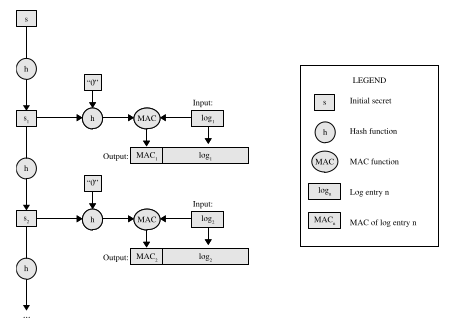
\includegraphics[scale=1]{imagenes/MAC.png}
\end{figure}
A la hora de verificar el estado de un registro en particular calculamos su clave en la cadena de hash.
Al log guardado le aplicamos la función de hash con la que obtenemos el MAC. Si este no coincide con el almacenado,
el registro fue modificado. La siguiente imagen corresponde al proceso de verificación:
\begin{figure}[H]
\centering
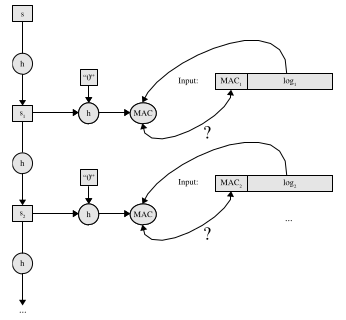
\includegraphics[scale=1]{imagenes/Verification.png}
\end{figure}
Omitimos la posibilidad de utilizar cifrado en los logs. Nos limitamos a señalar que se puede garantizar confidencialidad en el contenido de los registros utilizando cada secreto intermedio para encriptar el log, además de para generar su MAC.
Nuestra implementación tiene las siguientes particularidades:
\begin{itemize}
\item Utilizamos un secreto inicial, elegido por el administrador del equipo, para iniciar el servidor syslog.
Para cada log que se genere, se calcula su MAC y se guarda.
\item El propio administrador realizara la verificación de los logs aportando el secreto inicial.
\item Los registros de eventos se guardan en un ".log" de solo lectura para un usuario normal.
\item Cada verificación realiza el procedimiento descripto para todos los logs en el registro.
\end{itemize}
\subsection{Alternativas de diseño}
\subsubsection{Alternativas de diseño: Verificación acumulativa}
En lugar de guardar un MAC por cada registro del log, alternativamente se puede guardar solamente uno resultante de un calculo acumulativo. Este mecanismo consiste en que la función de hash toma no solamente la clave, sino también el MAC calculado anteriormente. 
Utilizando esto podemos guardar en un lado el registro de logs y, en otro, el último hash de la cadena. 

Existe un problema en la verificación acumulativa dado que necesita todos los logs previos para comprobar uno. Suponiendo que un atacante modifique el log borrando una parte de él, dejando registros previos y posteriores a la modificación intactos. Tanto el método de verificación que nosotros usamos como su versión acumulativa, podrán detectar el cambio. Además, los dos serán capaces de verificar que los logs previos al ataque están correctos y se puede confiar en ellos. Sin embargo, la verificación acumulativa es incapaz de saber si los registros posteriores están correctos.   
\subsubsection{Alternativas de diseño: Clave pública}
Una alternativa al uso de la cadena de hash consiste en firmar los logs utilizando una clave privada y verificar la firma con su clave pública. La principal ventaja de esta implementación es que permite que la verificación se pueda realizar con una clave diferente de la que se usa para firmar. 

El proceso consiste en generar un par de claves de los cuales se debe guardar de forma segura la publica(debe asegurar integridad). Utilizando la clave privada se firma una entrada del log que consiste en una secuencia de $n$ claves publicas utilizadas para verificar los $n-1$ siguientes logs. La última clave publica de la secuencia se utilizara para verificar la siguiente entrada que contendrá otra secuencia de claves publicas y así sucesivamente. Cada clave privada usada en la secuencia se descarta inmediatamente. El objetivo es tener las claves publicas a mano para la verificación y, dado que se están firmadas, se puede corroborar su autenticidad. En las siguientes imágenes se muestra el proceso de logging seguro.
\begin{figure}[H]
\centering
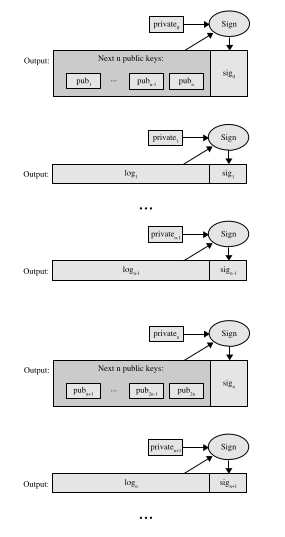
\includegraphics[scale=0.4]{imagenes/PublicKey.png}
\end{figure}
A la hora de verificar, se utilizara la clave publica inicial para el primer log que contiene la cadena de claves publicas. Si es correcto se verificaran cada uno de los siguientes $n$ logs utilizando esta secuencia. Se realizara el proceso para la siguiente entrada utilizando la última clave de la cadena y con esto se comprueba la siguiente cadena de claves publicas a utilizar para la verificación. La siguiente imagen ilustra el proceso.
\begin{figure}[H]
\centering
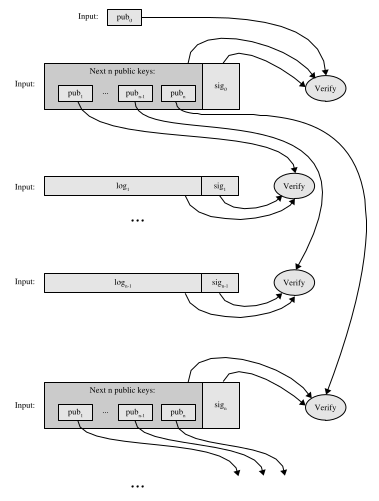
\includegraphics[scale=0.4]{imagenes/PublicKeyVerification.png}
\end{figure}
  
Además de la firma de los logs, se pueden utilizar las claves privadas para cifrar los logs, ocultando la información que contienen.
\subsubsection{Identity-based signature(IBS)}
Criptografía de curva elíptica: es una alternativa a RSA para generar pares de claves para criptografía asimétrica. La ventaja es que las claves generadas son cortar, ideales para las entradas del registro.

Identity-based signature es una alternativa al mecanismo asimétrico explicado anteriormente que permite obtener las claves públicas derivándolas de bits puntuales en un string y en la clave pública de un generador de claves privadas(PKG), la privada solo puede ser extraída de esa cadena de caracteres y de la clave privada del PKG. Con esto, lo que se necesita para la verificación es la siguiente clave pública del PKG. Con el otro modelo tenía que enumerar las claves públicas y pasarlas todas.
\subsection{Implementación}
\subsubsection{Instalación}
El server está programado en Python 2.7 y no tiene dependencias de librerías de terceros, por lo que ese el único requerimiento.
Descomprimiendo el zip con los fuentes en cualquier directorio alcanza como instalación.
Tampoco se necesitan permisos de root o de administrador para levantar el server porque por practicidad cambiamos el puerto estandard de syslog 514 a 5514.
\subsection{Uso}
Utilizando python se deberá ejecutar pysyslog.py para poner en marcha el servidor syslog, el cual pedirá ingresar un secreto que toma el rol del secreto inicial. 

\noindent
\begin{lstlisting}[language=bash,numbers=none]
  $ python pysyslog.py
\end{lstlisting}

La verificación se realiza ejecutando Verificacion.py, en la cual tenemos que aportar el secreto elegido anteriormente. Los registros se guardan en youlogfile.log. 

\noindent
\begin{lstlisting}[language=bash,numbers=none]
  $ python Verificacion.py
\end{lstlisting}

Para cargar un nuevo log basta con tener el server levantado en una consola, puerto 5514, y desde otra consola se puede enviar un paquete udp con netcat, así como lo haría otro servicio que loguee a cualquier otro syslog server.

\noindent
\begin{lstlisting}[language=bash,numbers=none]
  $ echo -n "Contenido del log" | nc -4u -w1 127.0.0.1 5514
\end{lstlisting}



